% coding:utf-8

%----------------------------------------
%FOSADSVB, a LaTeX-Code for a summary of digital signal processing
%Copyright (C) 2015, Mario Felder & Michi Fallegger

%This program is free software; you can redistribute it and/or
%modify it under the terms of the GNU General Public License
%as published by the Free Software Foundation; either version 2
%of the License, or (at your option) any later version.

%This program is distributed in the hope that it will be useful,
%but WITHOUT ANY WARRANTY; without even the implied warranty of
%MERCHANTABILITY or FITNESS FOR A PARTICULAR PURPOSE.  See the
%GNU General Public License for more details.
%----------------------------------------

\chapter{Adaptive Filter}
Der Wiener- und Kalman-Filter sind optimale Filter unter der Annahmen, 
dass die Statistik über des involvierten Zufallsprozesses komplett
bekannt sind. In der Praxis ist die üblicherweise nicht der Fall. 
Adaptive Filter passen sich unbekanntem und sich ändernder Umgebung 
automatisch an.
\section{Linear Predictive Coding (LPC-10e)} 
Statt die Wellenform zu codieren, bildet der Vocoder ein Modell und
extrahiert die Parameter davon.\\\\
Das menschliche Sprachsignal wird mit einem all-pole Filter nach dem 
AR-Modell mit Ordnung $P$ abgebildet:
\[ H(z) = \frac{g}{1-\sum_{k=1}^{P}a_k\cdot z^{-k}} \]
Die Anregung erfolt mit einem Impulskamm oder einem Rauschprozess.
LPC-10e Algorithmus:
\begin{itemize}[noitemsep,topsep=3pt]
	\item 8000 Samples/s
	\item 180 Samples/Segment
	\item Ordnung $P=10$
	\item 54 Bits pro Segment für Encoding
	\item Bitrate von 2400 Bit/s
\end{itemize}
Entscheidet für jedes Segment, ob es voiced oder unvoiced ist, berechnet die
Filterkoeffizienten $a_1, a_2,...,a_{10}$ und bestimmt das Gain $g$. Konsonanten 
zählen als unvoiced, da das Signal einem Rauschen gleicht. Vokale erzeugen eine 
periodische Schwingung mit $T_0$, welche pro Segment bestimmt wird.\\
\\
Differenzengleichung des unten ersichtlichen Systems:
\[ s[n] = \sum_{k=1}^{P} \bigg(a_k\cdot s[n-1] + g \cdot v[n]\bigg) \]
\begin{minipage}{.5\textwidth}
\begin{center}
	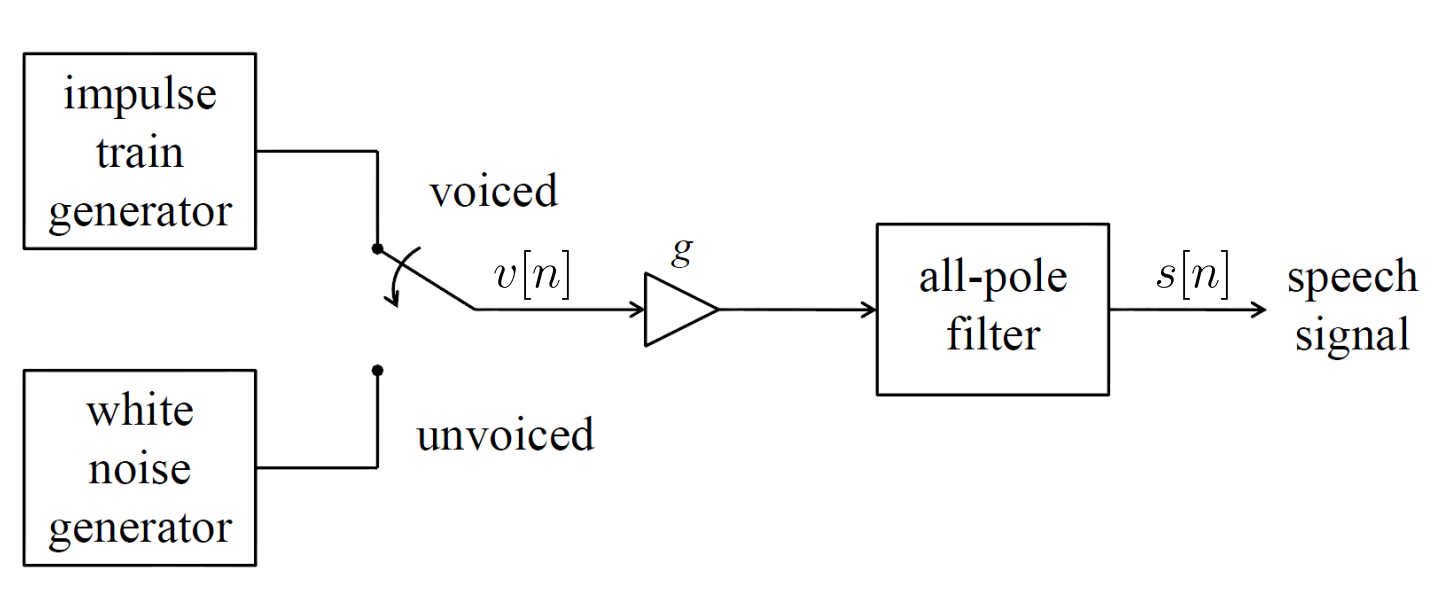
\includegraphics[width=\textwidth]{../fig/speech_signal}
\end{center}
\end{minipage}
\begin{minipage}{.45\textwidth}
\begin{center}
	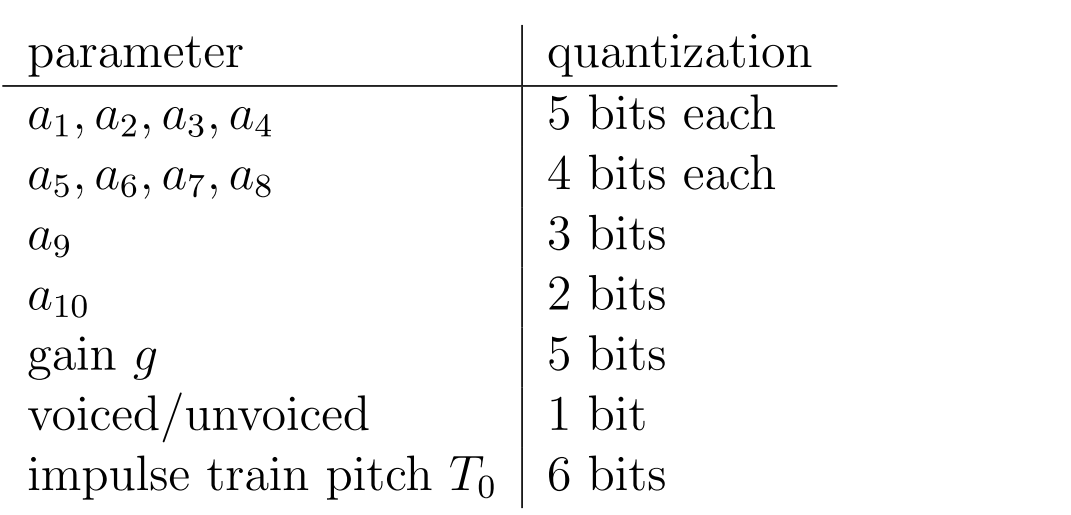
\includegraphics[width=\textwidth]{../fig/lpc_10e}
\end{center}
\end{minipage}
~\\
Die Parameter $a_k$ müssen so gefunden werden, dass der "'one step linear predictor"'
\[ \hat{s}[n] = \sum_{k=1}^{P}a_k\cdot s_{in}[n-k] \]
möglichst nahe an $s_{in}[n]$ kommt. Dazu kann die Wiener-Filter-Theorie angewendet werden, es ergibt sich also:
\[ \textbf{R}_{ss} = \begin{bmatrix}
	\gamma_{ss}[0]	& \gamma_{ss}[1]	& \ldots	& \gamma_{ss}[P-1]\\
	\gamma_{ss}[1]	& \gamma_{ss}[0]	& \ldots	& \gamma_{ss}[P-2]\\
	\vdots			& \vdots			&			& \vdots\\
	\gamma_{ss}[P-1]& \gamma_{ss}[P-2]	& \ldots	& \gamma_{ss}[0]
\end{bmatrix}, \qquad 
 \textbf{r}_{ss} = \begin{bmatrix}
	\gamma_{ss}[1]\\
	\gamma_{ss}[2]\\
	\vdots\\
	\gamma_{ss}[P]
\end{bmatrix} \quad \text{und} \quad \textbf{a} = \textbf{R}_{ss}^{-1}\cdot \textbf{r}_{ss} \]
Es wird also ein Predictor mit $D=1$ angewendet, $\gamma_{ss}[m]$ ist die Autokorrelation von $s_{in}[n]$.
Die Werte der Autokorrelation müssten angenähert werden durch:
\[ \hat{\gamma}_{ss}[m] = \frac{1}{N-m} \sum_{n=1}^{N-m}s_{in}[n]\cdot s_{in}[n+m], \qquad \text{biased Variante mit: } \frac{1}{N}\]
mit $N$ für die Anzahl Werte im Segment, beim LPC-10e also $N=180$.\\\\
Der Fehler beträgt und ist abhängig von der Verstärkung:
\[ d[n] = s_{in}[n]-\hat{s}[n] \]
Die Verstärkung ergibt sich nach:
\[ g=\sqrt{\frac{1}{N}\sum_{n=1}^{N}d^2[n]} \]
Zur Unterscheidung zwischen "'voiced"' und "'unvoiced"' sowie für den Pitch
wird die durchschnittliche Amplituden-Differenz-Funktion (average magnitude difference
function) verwendet, definiert als:
\[ \bar{\gamma}_d[m]= \frac{1}{N-m} \sum_{n=1}^{N-m}\left|\frac{d[n]}{g} -
	\frac{d[n+m]}{g}\right| \] 
Wenn das Minimum von $\bar{\gamma}_d[m]$ unter einen Schwellwert fällt, wird das
Segment als "'voiced"' deklariert:
\[ T_0 = \arg \min_{m\in[20,160]} \bar{\gamma}_d[m] \]

%===============================================================================
\section{LMS Algorithmus (least mean square)}
Passt seine Filterkoeffizienten sample-für-sample basierend auf dem Fehler $s[n]-\hat{s}[n]$ an.
Eignet sich beispielsweise für die Echo-Cancellation in der Telefonie. Beim variablen Filter handelt  
es sich oft um einen FIR-Filter.
\begin{center}
	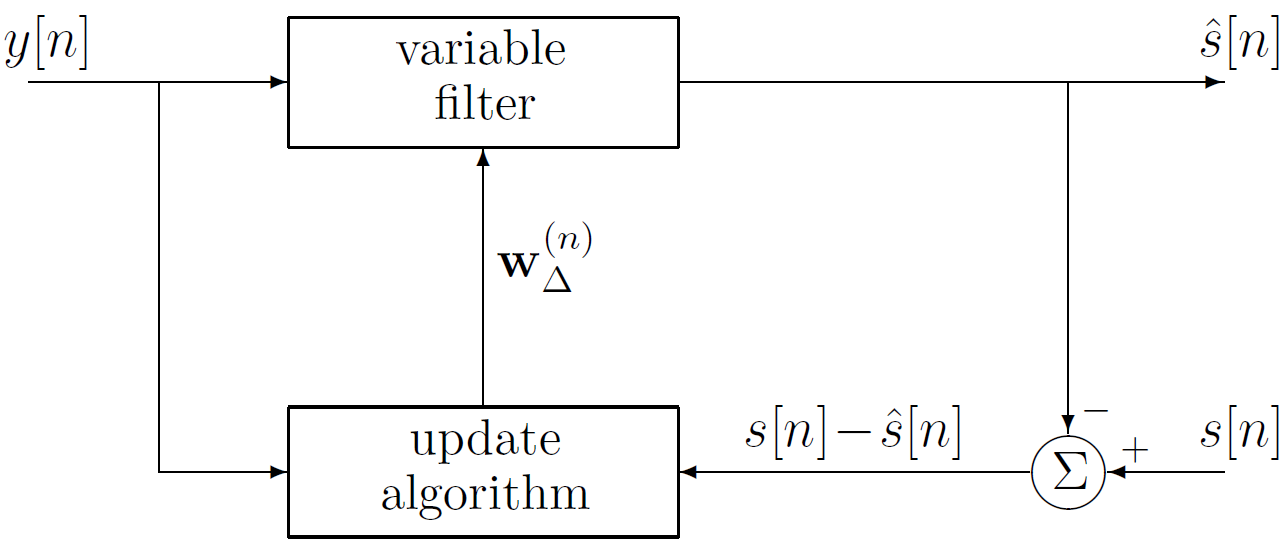
\includegraphics[width=.525\textwidth]{../fig/lms_adaptive_modell}
\end{center}
Das Filter schaltet von einem Training-Modus, in dem die Preamble einer Nachricht analysiert wird,
in den Entscheidungsmodus um, in dem die Nutzdaten ausgewertet werden.\\\\ 
Es wird der Eingangvektor und die Filterkoeffizienten benötigt:
\[ \textbf{y}_n = \begin{bmatrix}y[n] \\ y[n-1] \\ \vdots \\ y[n-M]
	\end{bmatrix} \qquad \textbf{w} = \begin{bmatrix}
		w_0 \\ w_1 \\ \vdots \\ w_M	\end{bmatrix} \]
Der Ausgang des variablen FIR-Filters wird berechnet mit:
\[ \hat{s}[n] = \textbf{w}^T\cdot \textbf{y}_n \]
Der mittlere quadratische Fehler ist:
\[ \varepsilon_{MSE}(\textbf{w}) = E \{ (\hat{s}[n]-s[n])^2 \} \]
Der Vektor \textbf{w} wird zu Beginn mit $M+1$ Nullen initialisiert und berechnet sich danach aus:
\[ \textbf{w}^{(n+1)} = \textbf{w}^{(n)} + \underbrace{\mu\left( s[n] - 
	\left( \textbf{w}^{(n)}\right)^T\textbf{y}_n\right)\cdot\textbf{y}_n}_
	{=\textbf{w}_\Delta^{(n)}} \]
$\mu$ ist die Schrittweite und. Ein zu kleiner Wert resultiert in einer langsamen Anpassung, 
ein zu grosser Wert kann zu Schwingungen um das Optimum herum führen.\\\\
Im folgenden sind die Verläufe des Fehlers bei verschiedenen Schrittweiten $\mu$ aufgezeichnet.
Es soll ein mit weissem Rauschen $v[n]$ überlagertes Signal $s[n]$ gefiltert werden. Das Filter
hat Ordnung $M=12$ und startet mit $\textbf{w}$ als Nullvektor. Mit steigender Anzahl Samples 
verringert sich der Fehler und kommt immer näher an den optimalen Filter (Wiener-Filter) heran.\\\\
Bessere Resultate (schnellere Konvergenz) wären mit einem RLS-Filter erzielbar. 
Dieser weisst jedoch eine deutlich höhere Komplexität auf als der LMS-Filter.
\begin{center}
	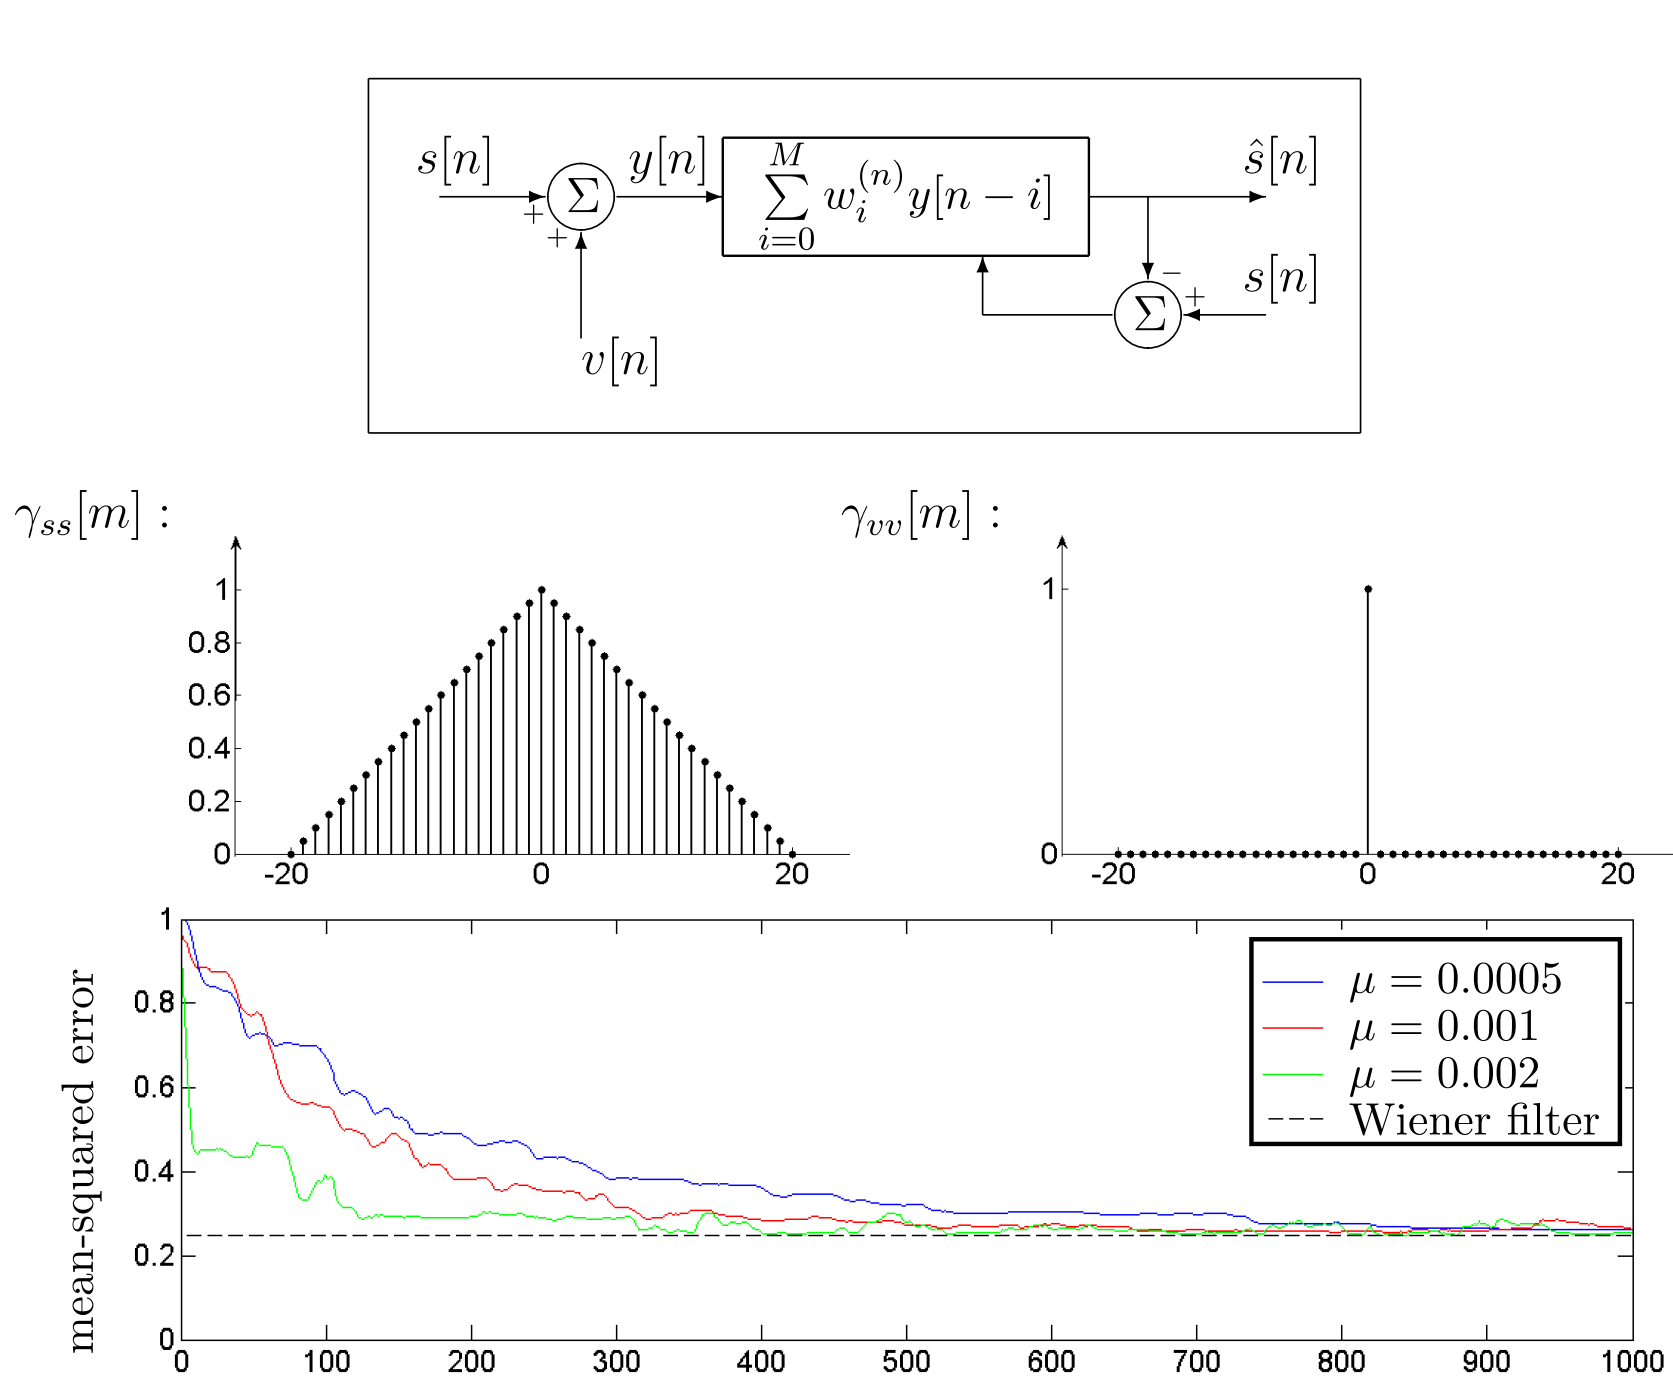
\includegraphics[width=.7\textwidth]{../fig/lms_algorithm}
\end{center}
\newpage

%===============================================================================
\section{Echo cancellation}
Konferenztelefone müssen das Echo, welches durch das vom Lautsprecher ausgestrahlte Audiosignal 
vom "'anderen Ende der Leitung"' entsteht und erneut vom Mikrophon aufgenommen wird, herausfiltern 
können. Für diese Aufgabe wird typischerweise ein adaptives Filter eingesetzt. 
\begin{center}
	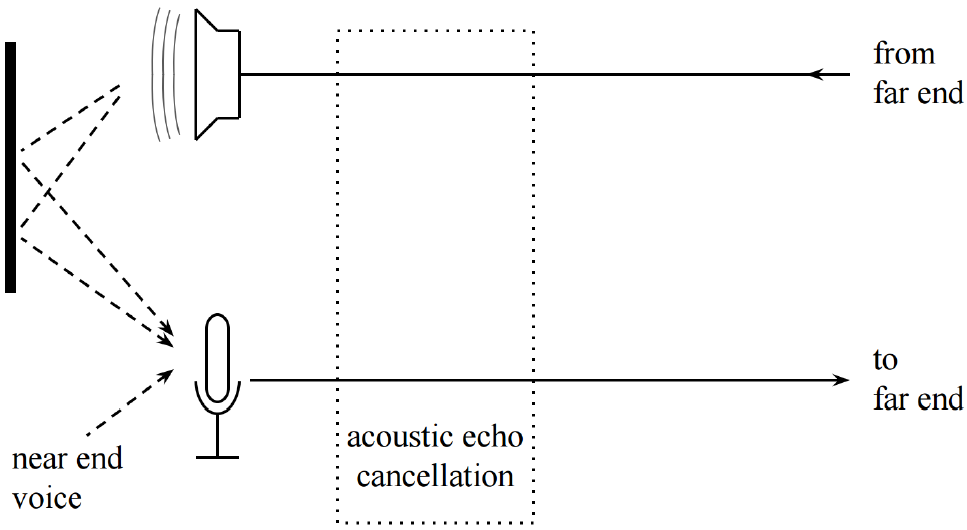
\includegraphics[width=.5\textwidth]{../fig/echo_cancellation}
\end{center}
$H(z)$ repräsentiert den Pfad zwischen Lautsprecher und Mikrophon inklusive allen möglichen Pfaden, 
welche die Schallwellen nehmen können. Es kann mit einem LTI-System modelliert werden. $H(z)$ 
versucht, das verzerrte Signal nachzubilden, welches vom Mikrophon wieder aufgenommen wird. 
\begin{center}
	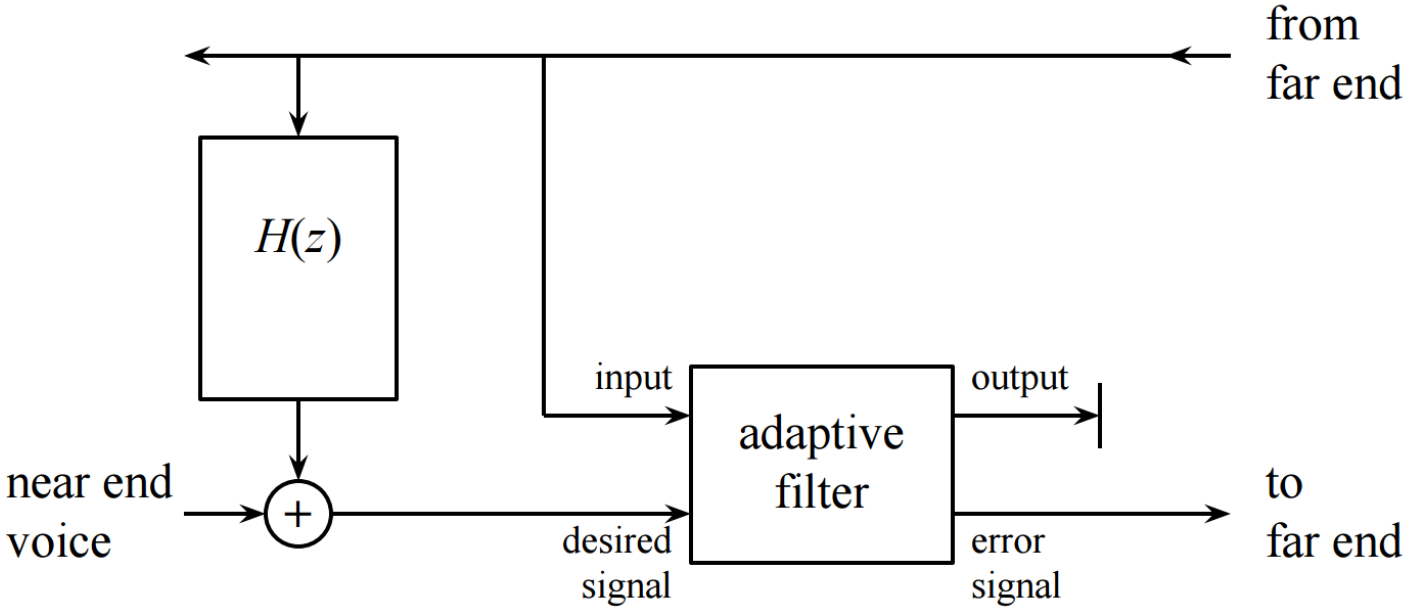
\includegraphics[width=.5\textwidth]{../fig/echo_cancellation_modell}
\end{center}
Das obige Modell wird erweitert, in dem unterschieden wird, ob eine Person spricht (am jeweiligen Ende), 
oder ob beide Personen sprechen. Ohne Unterscheidung verschlechtert sich durch das Filter die Qualität
des Audiosignals. Einige Systeme fügen "'comfort noise"' hinzu. So bleibt die Gegenseite nicht komplett
still, was für den Menschen ungewohnt ist. 